\documentclass[12pt,notitlepage]{article}
\usepackage[bitstream-charter]{mathdesign}
\usepackage{inconsolata}
\usepackage[T1]{fontenc}
\usepackage{microtype}
\usepackage[utf8x]{inputenc}
\usepackage[letterpaper,margin=1in]{geometry}
\usepackage{titlesec}
\usepackage{graphicx}
\usepackage{wrapfig}
\usepackage{caption}
\usepackage{subcaption}
\usepackage{hyperref}

\newcommand\footnoteref[1]{\footnote{\url{#1}}}
\newcommand\tmts[0]{\texttt{tell me to survive}}

\titleformat{\section}{\normalfont\large}{\thesection}{0.5em}{}
\titleformat{\subsection}{\bfseries}{\thesubsection}{0.5em}{}
\titleformat{\subsubsection}{\normalfont}{\thesubsubsection}{0.5em}{}
\titlespacing*{\section}{0em}{0.75em}{0.3em}

\begin{document}
\begingroup
  \centering
  {\Large \texttt{tell me to survive}: Concreteness Fading and Visual
    Programming in Teaching Object-Oriented Programming\\[1em]}

  Andy Jiang, Michael Mauer, and David Li\par
\endgroup

\section{Introduction and Motivation}

Much effort has gone towards methods to teach programming as an
overall concept, with systems like Alice, Scratch, and CodeSpells
demonstrating how visual programming can successfully introduce
students to this field. Our goal is to teach the more specific topic
of object-oriented programming to novice programmers using these same
techniques, focusing on how to abstract and represent ideas such as
method definitions, subclassing, and overriding in such a framework.
Additionally, to reinforce these concepts to an audience already
somewhat familiar with programming, we will introduce concreteness
fading to the system, transitioning students from visual programming
to directly writing code. This will facilitate the learning of these
specific higher-level concepts and abstractions within computer
science, which is important to effectively educate and train the next
generation of computer science and software development students.

\section{Related Work}

The idea of visual programming manipulating robots or other objects in
a virtual world is not a new one; we list several games and projects
in the same vein, with some comparison to our project.

\begin{itemize}
\item CodeSpells\footnoteref{https://codespells.org/}
\item Scratch\footnoteref{https://scratch.mit.edu/}/Alice\footnoteref{http://www.alice.org/}
\item Looking Glass\footnoteref{https://lookingglass.wustl.edu/}
\item Hour of Code\footnoteref{https://code.org/learn}
\item LightBot\footnoteref{https://lightbot.com/hocflash.html}
\item Human Resource Machine\footnoteref{https://tomorrowcorporation.com/humanresourcemachine}
\item Blockly Games\footnoteref{https://blockly-games.appspot.com/}
\item BlockPy\footnoteref{https://github.com/RealTimeWeb/blockpy}
\end{itemize}

CodeSpells, Alice, Scratch, and Looking Glass are more free-form;
instead of specific puzzles or levels to solve, they simply place the
player in a sandbox. Looking Glass tries to come up with metaphors for
object-oriented concepts, and manages to cover more of them than our
project does, but does not employ concreteness fading. Hour of Code,
LightBot, and Human Resource Machine take the same puzzle-oriented
approach our game does, but also lack the concreteness fading
aspect. Blockly Games is the most similar to our approach, initially
using blocks whose labels transition from text descriptions to code,
then changing to a text editor at the end. However, it does not
present a consistent game, changing the theme and mechanics of the
game every few levels. BlockPy is more advanced, enabling the player
to seamlessly switch between code and visual programming (and
translating one to the other), but does not use concreteness fading
either.

\section{Methodology}

\tmts{} is a purely client-side, web-based game built on
HTML5/JavaScript using Python as its instructional language. The core
concept is manipulating robots in a game world via visual or
text-based programming in order to solve puzzles and accomplish
certain objectives.

\subsection{Concepts}

\subsubsection{Learning Goals}

\begin{figure}[h]
  \centering
  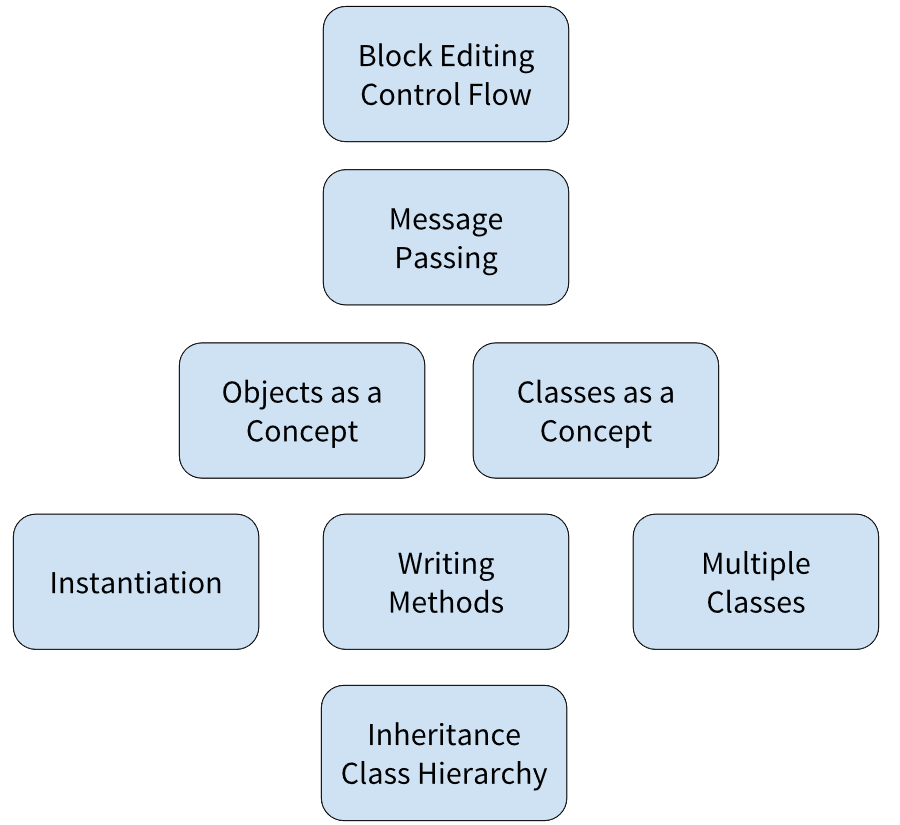
\includegraphics[width=.6\textwidth]{progression}
  \caption{Concept Progression}
\label{fig:progression}
\end{figure}

We limited our scope to the concepts in \autoref{fig:progression} in
order to limit the game length and complexity, and because of
implementation constraints. This means that advanced topics such as
abstract classes and polymorphism are not covered. This is an
acceptable trade-off because the purpose of this game is not to teach
OOP in its entirety, but rather to ease the conceptual transition for
new programmers.

\autoref{fig:progression} lists the progression of requisite skills up
to mastery of inheritance (our overall learning objective). Mastering
a skill in any given level in the diagram should require mastering
every skill in the previous level. For instance, using inheritance
effectively requires that the user is writing methods across several
classes in the hierarchy, then instantiating different types of objects
with those classes. These individual skills can then be further subdivided
down to the basics of using our click-and-drag block input system.


\subsubsection{Concept Progression}

Key to helping players master concepts is the order and pace at which
they are presented. Thus, we spent quite a bit of time trying to build
up a level progression which slowly moves concept by concept through
the skill tree in \autoref{fig:progression}. The basic premise is that
there should only be about 1 new concept per level; otherwise, users
are likely to get confused. One of the predominant ways this manifests
in our game play is the introduction of new robots. Different robots
introduce ideas related to inheritance. At first this is as simple as
identifying that MineRobot (and other subclasses) can use functions
for moving and turning from the basic Robot class. However, there are
more complex applications later on, such as the way that FrackingRobot
overrides a function from MineRobot. Moreover, as new concepts are
introduced, old concepts are recombined to make new puzzles. For
example, the HeavyLifter is used in a context such that it needs to
use a function defined in the basic Robot class. However, it also
requires implementing that method first.

\subsubsection{Concreteness Fading}

Of course, the progression of actual concepts works in tandem with the
gradual concreteness fading of the actual blocks that the user is
working with. A key issue here, which we identified in user tests
during the beta phase, is that changes to the blocks should not happen
while another concept is introduced because players get overwhelmed by
the number of new skills required. Thus, we have some levels where we
introduce no new object-oriented concepts. Instead, we pose a simpler
puzzle focusing on usage of the newly faded block.

Our fading process has 3 stages. Initially, all blocks start off as
textual descriptions of what they do, e.g.\ ``tell \_ to \_'' for
method invocation or ``create a new \_ called \_'' for object
instantiation (see \autoref{fig:block-unfaded}). As the player
progresses, the labels on the blocks are faded into actual Python code,
as in \autoref{fig:block-faded}. Eventually, the player will be given
a text editor and asked to write the Python code themselves. Some
scaffolding always remains; for instance, the object hierarchy view always
remains accessible after it is introduced, and serves as a reference for
what classes and methods are available.

\begin{figure}[h]
\centering
\begin{subfigure}{.5\textwidth}
  \centering
  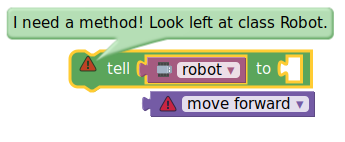
\includegraphics[width=.5\textwidth]{block_unfaded}
  \caption{An unfaded method invocation block.}\label{fig:block-unfaded}
\end{subfigure}%
\begin{subfigure}{.5\textwidth}
  \centering
  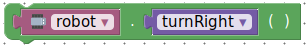
\includegraphics[width=.5\textwidth]{block_faded}
  \caption{The faded method invocation block.}\label{fig:block-faded}
\end{subfigure}
\label{fig:test}
\end{figure}


\subsection{Application Design}

A key factor motivating our design was a constant process of
simplification, driven by user testing. For example, at first for
loops had a corresponding number block that needed to be placed in the
loop. This was rather tedious, so we changed it to a basic text input
box instead. We also decided not to provide more complicated control
flow, such as boolean logic and other types of loops. In fact, even
the tell blocks are greatly simplified. Notice that no functions take
parameters or return values. Our goal was to focus more on a basic set
of OOP concepts and the corresponding syntax. Thus, we limited access
to features that would increase the complexity of solution
code. Instead, solutions are reliant on understanding key OOP
concepts.

The memory limit in each level is another example of this
restriction. Similar to the way LightBot forces players to define
functions due to lack of space, we also design levels such that there
is no way to finish under the memory limit without defining a
method. This forces players to consider the class hierarchy and
actually implement methods they call on objects. Without this
restriction, the hierarchy (and thus our goal of teaching OOP) could
potentially be disregarded.
% TODO: did we find a user that actually did that?

\subsection{Evaluation}

We evaluated the performance of the game by administering a pre-test
and post-test to all people who completed the game.

\subsubsection{Audience}

We targeted students who are currently enrolled in or have taken only
an introductory programming course. The game was advertised in CS 1110
(Spring 2016) at Cornell, and at Sparta High School, as well as
to specific students who have taken CS 1110 here.

\section{Results}

\subsection{Pre- and Post-Test}

The Pre- and Post-Tests that we gave were identical, 5 question quizzes
testing both object-oriented python syntax and general concepts. The goal
was to present questions that test for both practical and more abstract
understanding. The quizzes were strongly integrated into the game itself,
presented as an ``Robot Commander Aptitude Test'' and a ``Robot Commander
Proficiency Test''.

\subsection{Subjective Impressions}

\subsection{TODO}

\section{Conclusions}

\end{document}
